% 
% Annual Cognitive Science Conference
% Sample LaTeX Paper -- Proceedings Format
% 

% Original : Ashwin Ram (ashwin@cc.gatech.edu)       04/01/1994
% Modified : Johanna Moore (jmoore@cs.pitt.edu)      03/17/1995
% Modified : David Noelle (noelle@ucsd.edu)          03/15/1996
% Modified : Pat Langley (langley@cs.stanford.edu)   01/26/1997
% Latex2e corrections by Ramin Charles Nakisa        01/28/1997 
% Modified : Tina Eliassi-Rad (eliassi@cs.wisc.edu)  01/31/1998
% Modified : Trisha Yannuzzi (trisha@ircs.upenn.edu) 12/28/1999 (in process)
% Modified : Mary Ellen Foster (M.E.Foster@ed.ac.uk) 12/11/2000
% Modified : Ken Forbus                              01/23/2004
% Modified : Eli M. Silk (esilk@pitt.edu)            05/24/2005
% Modified: Niels Taatgen (taatgen@cmu.edu)  10/24/2006

%% Change ``a4paper'' in the following line to ``letterpaper'' if you are
%% producing a letter-format document.






%%%% Remaining todos
% add more discussion
% add figure for Expt 3 results?
% overall proofreading
% have a better title

\documentclass[10pt,letterpaper]{article}

\usepackage{cogsci}
\usepackage{pslatex}
\usepackage{apacite}
\usepackage{graphicx}
\usepackage{color}
\usepackage{amsmath}

\definecolor{Red}{RGB}{255,0,0}
\newcommand{\red}[1]{\textcolor{Red}{#1}}  

\title{ When does a near-miss sting? }
 
\author{{\large \bf Desmond C. Ong (dco@stanford.edu)} \\
{\large \bf Jamil Zaki (jzaki@stanford.edu)} \\
{\large \bf Noah D. Goodman (ngoodman@stanford.edu)} \\
  Department of Psychology, Stanford University, Stanford CA, USA 
}

\begin{document}

\maketitle

\begin{abstract}
Observers often judge agents to be more unhappy when the agents miss a desired outcome by a small margin, compared to a large margin. This has been shown in situations where the agents have control over the outcome, such as in missing planes. Here, we show that intuitive theories of emotion incorporate near-misses even for events with randomly-determined outcomes, and this might be due in part to the illusion of control over random events. Finally, we integrate near-misses into a more general model of affective cognition, and quantify the psychological cost of a near-miss relative to winning and losing.

%Near misses---missing a desired outcome by a small margin---are more emotionally intense than normal misses, even though the outcomes tend to be no different, and people readily accord near-miss effects when reasoning about others. Yet there are still open questions: what are the distance dimensions along which near misses are judged, and how do people incorporate near misses into more general affective cognition, or reasoning about emotion? In this paper we show that intuitive theories of emotion seem to weigh near-misses even for random events, and this is driven by the semblance of action-outcome contingency. Finally, we incorporate near misses into a more general model of affective cognition, and quantify the psychological cost of a near-miss relative to winning and losing.

\textbf{Keywords:} 
Near Miss; Counterfactual Distance; Lay Theories; Emotion
\end{abstract}


\begin{quote}
\textit{``Close only counts in horseshoes and hand grenades"} 
--- English Idiom
\end{quote}

%Evidence suggests that contrary to the above idiom, close counts---\textit{emotionally}.


	When Rob achieves a desired outcome, such as winning a soccer match, we intuitively know that he would feel positive. Conversely, when Rob loses, or otherwise fails to achieve an outcome, we can reason that he would feel negative. Such intuitive reasoning about emotions comprises \textit{affective cognition} \cite{OngAffCog}, and forms an integral part of our social lives. Our intuitive theories of emotion, however, are more complex than considering just simple winning and losing: If Rob just fails to achieve the outcome by a small margin---a \textit{near-miss}---such as losing a soccer game by a single goal, we intuitively recognize that he actually would feel worse than if he had missed by a larger margin, because the outcome was ``so close" to winning. Penalty shootouts in soccer provides the most exaggerated of such near-miss scenarios: the losing team often loses because of one missed ball, sometimes an inch shy of escaping the goalkeeper's hands. These details add much more emotional intensity to all agents involved, more so than just a simple loss. Contrary to the above idiom, close \textit{does} count---\textit{emotionally}.
	
	Psychologists have long known that near-misses form an integral, but surprisingly not well understood part of affective cognition, or reasoning about emotions \cite{Johnson1986, Gleicher1990, Teigen1996}. Most of this work falls under the broader category of counterfactual thinking, or thinking about ``what might have been" \cite{Bryne2002,McMullen2002, Medvec1997, Roese1997}. Near-miss counterfactuals are particularly engaging, because these possible worlds almost happened: they were separated from the current world by some small ``distance". Consider \citeA{Kahneman1982}'s classic example of Mr Tees, who missed his plane by 5 minutes, and Mr Crane, who missed his plane by 30 minutes. People consistently judge the person who narrowly missed his plane to feel much worse than the one who missed it by a wider margin.
	
	
%	\red{NDG: here starts the more precise stuff. note: the notion of emotion attribution and tie ins to ToE should have already appeared. need to be more precise about what you mean by causally-relevant.}

	There however, remains many open questions regarding the nature of the near-miss effect in observers' lay theories of emotion. First, why does the near-miss effect hurt? One explanation is that agents (the targets of observers' reasoning) experiencing a near-miss could have done something different to achieve the desired outcome, increasing feelings of regret \cite<e.g.,>{Zeelenberg1998}. For example, Mr Tees could have left his home slightly earlier, and might have caught his plane then. Agents can exercise control over the situation, and thus could have affected the outcome. Indeed, previous work has shown, for example, that the controllability of (non-near-miss) outcomes affects counterfactual thinking (whether upward or downward counterfactuals are generated) \cite{Roese1995}. If near-misses are judged to hurt because of an agent's potential to have changed the outcome via a different action, then observers should only attribute near-misses to agents in situations where agents have control. This account should then predict that observers should not attribute near-miss effects when the outcome is outside the agent's control, such as in games of chance or other random events. That is, observers should not rate agents as feeling worse if the agents miss a demonstrably random goal by a small, compared to large, distance. Anecdotally, however, one might be able to think of people who narrowly missed winning a prize in a raffle, lottery, or lucky draw, as feeling bad because they ``just missed" winning. Previous work has also shown that gamblers showing increased motivation and persisting in gambling more after near misses, even though the outcome of games like slots are independent of the gambler's actions \cite{Kassinove2001, Reid1986}. In Experiment 1, we sought to test this further by examining whether observers incorporate near-misses in their judgments of others' emotions even in random scenarios. We show that observers readily judge an agent who ``narrowly misses" on a die game (by rolling a number close to the target number) to feel worse than one who misses by a larger amount, even though outcomes on a die game are not ordered like the number line.

	Second, when presented with multiple possible types of distances in random situations, how do observers weight these types of distances in their affective judgments? In any particular situation, there could be more than one \textit{dimension} of closeness. For example, if Rob narrowly loses a soccer game by one goal, one might consider distance along physical space (how physically close his goal attempts came to scoring), or along time (if the goal against his team came in the last few minutes of the game), just to name several dimensions. If we return to our discussion on games of chance, however, there could be several such dimensions as well, all of which are still out of the agent's control. One hypothesis is that observers might judge agents to feel some sort of ``illusory" control over games of luck (like the ``hot hand fallacy" or ``gambler's fallacy" that people use in judgments of winning probability, e.g., \citeNP{Roney2009}), and hence incorporate near-misses along those dimensions. Given multiple dimensions, this hypothesis would predict that observers would weight dimensions along which the agent has more illusory control over other dimensions. To illustrate this concretely, imagine that one was flipping over numbered cards trying to match a given target number. In this case, the agent has control over the position of the picked card, even though the number on the back of the card was out of his control. If he loses, there are thus two distances at play: the physical distance of the picked card to the target card, and the ``numerical distance" from the picked card to the target card. Our prediction would be that because the agent has control over the physical position of the picked card, observers would weight near-misses along physical proximity more than near-misses along numerical closeness. By contrast, if the game was slightly changed to be guessing the number behind a target card, and after the agent picks a number, the card holding the picked number was revealed. In this case, the agent has control over the number, and so we predict that observers would weight near-misses along numerical closeness more than along physical closeness. One might argue that physical closeness in the latter game is irrelevant, but so is numerical closeness in the former game. In fact, if the games were truly random, both dimensions in both versions of the game are out of the agent's control\footnote{In the former version where the agent picks the position of a card, and if the agent picks the card next to the winning card, one can imagine the agent generating the counterfactual ``oh if only I had picked the neighboring card". However, if the cards were truly randomly dealt and the agent repicked the neighboring card, he would still have had the same uniform chance of winning. One can consider an analogy to re-rolling a dice; the outcome is still randomly-generated.}. In Experiment 2, we directly test this hypothesis of illusory control, and show that observers incorporate larger near-miss effects along dimensions that the agent has illusory control over.

	Finally, how much does a near-miss cost psychologically? That is, what is the size of the near miss effect (narrowly missing a desired outcome) relative to the happiness of actually obtaining said desired outcome? In Experiment 3, we build upon a previous model of affective cognition \cite{OngAffCog}. This model used a gambling paradigm that allowed us to parametrically vary features of the situation that affects judgment of emotions, such as the payoff structure and the distance to the neighboring outcomes. We explicitly incorporate modeling of near-miss effects into this existing quantitative model, which allowed estimates of the relative effect sizes and a better quantitative understanding of near miss judgments. More importantly, this enables the integration of near miss emotional judgments into existing models of affective cognition, and allows the construction of more comprehensive models of affective cognition.  

	In summary, this paper makes three contributions: we explored (i) whether people incorporate near-misses in their intuitive theories of emotion for scenarios with randomly-determined outcomes; (ii) whether people might do so because of the illusion of control over these outcomes; and (iii) how much near-misses cost relative to winning and losing, via incorporation of near-misses into a quantitative model of affective cognition.








%%%%


\section{Experiment 1: Near Miss effects in a random event}

In Experiment 1, we tested if participants would incorporate near-miss effects in their judgment of emotions when agents were playing a luck-based die-rolling game. Importantly, we measured near-misses along numerical closeness, and because the outcomes from rolling dice are completely random, the agent does not have control over the outcome.
%, and so the numerical closeness of the outcome compared to the desired outcome is not relevant. \red{NDG: i tweaked this \P, but should be adjusted based on how we clarify causal relevance in intro.}

\subsubsection{Participants.} We recruited 150 participants through Amazon's Mechanical Turk.

\subsubsection{Procedures.} Participants read about two characters, Jacob and Alex, who were playing a gambling game. Both needed to roll a 6 on a die to win. Jacob rolled a 1, while Alex rolled a 5. Participants then answered attention check questions (``what did X roll?") before attributing emotions along six categories (\textit{happiness}, \textit{sadness}, \textit{relief}, \textit{regret}, \textit{contentment} and \textit{disappointment})  to each character. Finally, they answered a three-alternative forced choice question: ``Who felt worse?", and were allowed to endorse ``They both felt equally bad" as an option. Participants were prompted for a free-response justification for their choice.

\subsubsection{Results.} Three participants were excluded for failing the attention check. Participants rated the near miss character (the character who rolled the 5) as feeling significantly more disappointed ($t(146)=2.17, p=0.03$), but no different on the other emotions. In the forced-choice question, a large majority (107/147 = 73\%) rated both characters as feeling equally bad. Among the remaining participants, significantly more participants rated the character who rolled the 5 (the near miss character) as feeling worse (N=30) compared to the character who rolled a 1 (N=10; exact binomial test $p=.002$; bootstrapped simulation with 10,000 iterations on full sample, $p=0.0007$) (See Fig. \ref{Expt1ResultFig}.)

\begin{figure}[htb!]
\includegraphics[width=\columnwidth]{images/Expt1results.png}
\caption{ Expt 1 Results. Proportions of forced choice response. Error bars indicate standard errors. The goal was to roll a ``6". More people judged the character who rolled a ``5" as feeling worse than the character who rolled a ``1".}
\label{Expt1ResultFig}
\end{figure}

To gain further insight into participants' judgments, we analyzed their free-response justifications and coded them into three categories. 84 (57\%) participants made their judgments based on equal outcomes (e.g. ``they both lost so they should feel equally bad"), 40 (27\%) participants made reference to closeness (e.g. ``he was soooo close"), and only 22 (15\%) participants made an explicit reference to there being no closeness difference (``it's a 1/6 chance for both of them"; ``the numbers are meaningless"). 1 participant chose not to give a justification. 

Thus, we find that while a large majority of participants said that both characters felt equally bad, this is primarily due to the fact that both characters lost. Perhaps, the emotions due to the near-miss effect are smaller in magnitude than the emotions resulting from the loss, and so for these participants, the near miss difference was not above their threshold to endorse a difference in emotional valence. Interestingly, of the participants who made any remarks on closeness or the lack thereof, the majority actually remarked that there \textit{is} a subjective feeling of closeness. This suggests that some observers are sensitive to near-miss effects in this scenario and they (irrationally) judge near-misses based on a randomly-determined distance that the agent has no control over.


%Thus, we find that while a large majority of participants said that both characters felt equally bad, this is primarily due to the fact that both characters lost. This is in line with our predictions \red{[NDG: i'll like this better when the predictions feel less ad hoc in intro..]} that the near-miss effect is much smaller in magnitude than the actual utility derived from the loss, and perhaps for these participants, the near miss difference was not above their threshold to endorse a difference in emotional valence. Interestingly, of the participants who made any remarks on closeness or the lack thereof, the majority actually remarked that there is a subjective feeling of closeness. This suggests that some observers are sensitive to near-miss effects in this scenario and the majority (irrationally) judge closeness based on a causally-irrelevant dimension.







\section{Experiment 2: Changing the dimensions of illusory control in random events}

We designed Experiment 2 to investigate weighting of closeness effects along different dimensions in a random game. Using a card guessing task, we manipulated the illusion of control of either the positions of the cards or the numbers on the cards, and showed that near-miss effects along the dimension with illusory control are more strongly incorporated into observers' lay theory of emotion. 


\subsubsection{Participants.} We recruited 200 participants through Amazon's Mechanical Turk, and assigned them to one of two conditions: Choose-Position (\textit{Pos}; N=100) and Choose-Number (\textit{Num}; N=100)



\subsubsection{Procedures.} 

\begin{figure}[htb!]
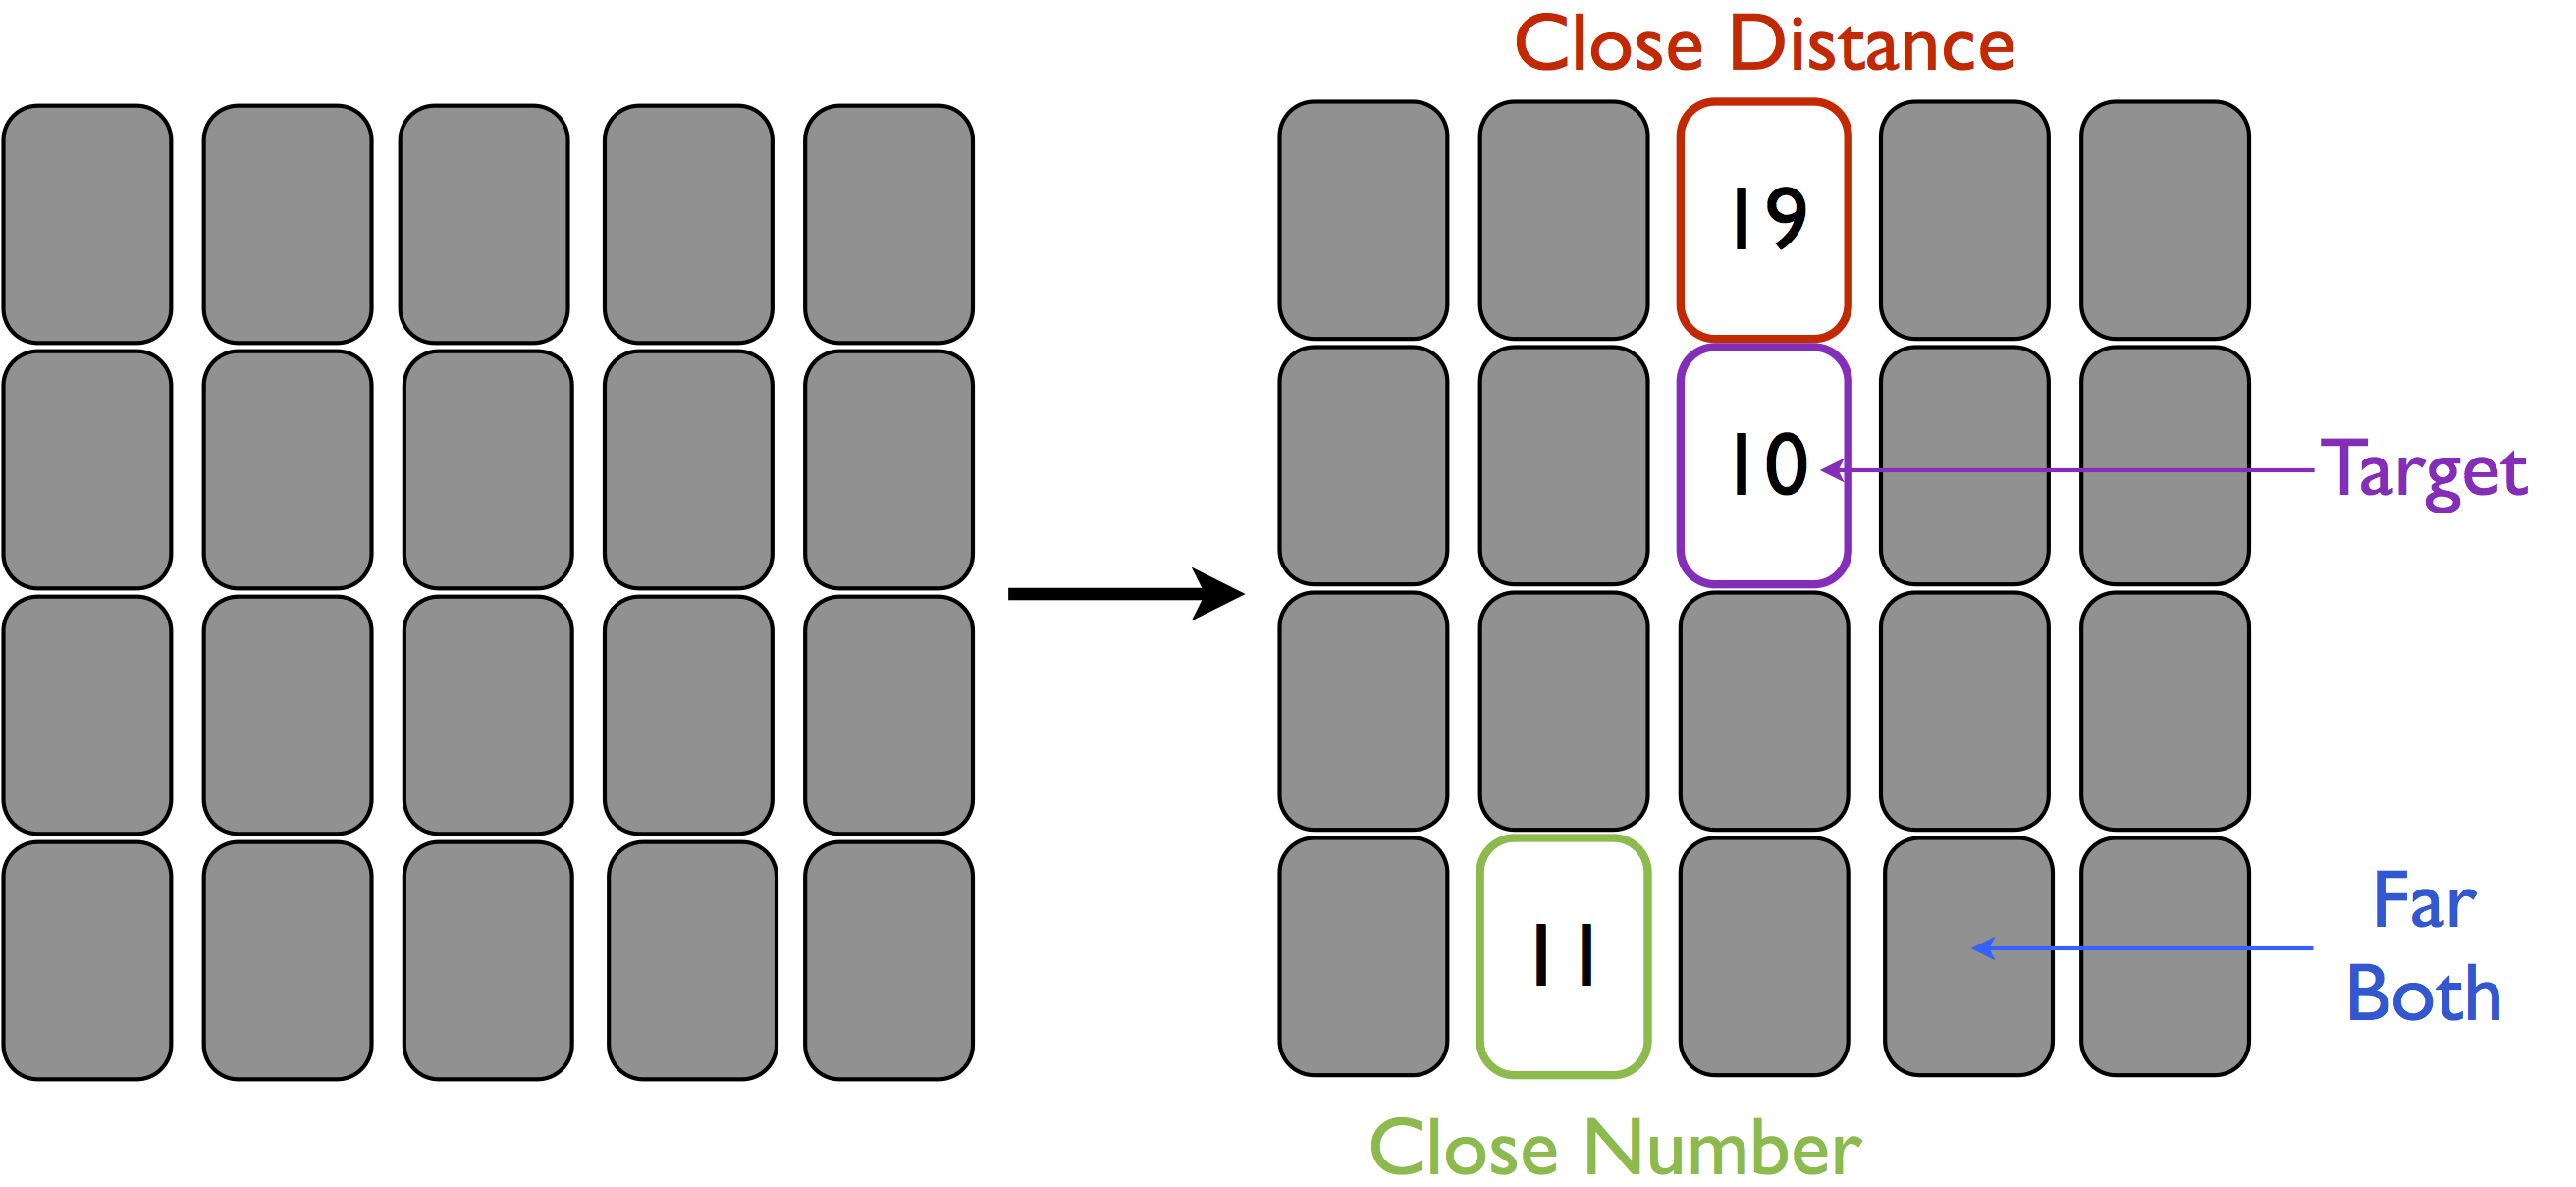
\includegraphics[width=\columnwidth]{images/card_paradigm.png}
\caption{ Expt 2 Paradigm, \textit{Pos} condition. Characters' goal is to pick the card with the 10. In the critical trial, the characters pick 19, in red, which is \textbf{close} in \textbf{distance}, and 11, in green, which is \textbf{close} in \textbf{number}. The target card, 10, is then revealed (outlined in purple). In other trials, one of the cards picked might be the number 1 (indicated by the blue arrow), which is \textbf{Far} in both distance and number. }
\label{Expt2ParadigmFig}
\end{figure}


In the Choose-Position (\textit{Pos}) condition, participants saw a 5x4 array of cards face down. They were told that two characters were playing a game: the cards were numbered 1-20, and they had to pick the card with the number 10 to win. There were three types of trials, which are all between subject manipulations, and each participant only saw one trial. In the ``Close Distance vs. Close Number" trial (depicted in Fig. \ref{Expt2ParadigmFig}), participants were told of two characters, Scott, who picked 19 (close distance), and Frank, who picked 11 (close number). After the characters picked their cards, the winning number 10 is revealed. Participants saw the locations of the two cards as well as the winning card. The close distance character's card was only 1 card away (in physical distance) from the winning card, while the close number character's card had a number that was only 1 away (in numerosity) from the winning card. Participants then rated the emotions of the two characters they saw (along the same six emotions as Expt 1). Finally, participants answered a forced-choice question, ``Who felt worse?", with the option to say ``Both felt equally bad."

The two other trials included a control character for comparison. In the ``Close Distance vs. Far Both" comparison, participants saw Scott (who picked the 19 card) and David, who picked a card with 1 on it, which is far along both physical distance and numerosity. In this case, David's card is 9 numbers away from the winning card, which is the same as Scott. In the ``Close Number vs. Far Both" comparison, participants saw Frank (who picked the 11 card) and David. In this case, David's card is just as far in physical distance from the winning card as Frank's card.


In the Choose-Number (\textit{Num}) condition, participants were presented with slightly different rules of the game. There were the same 20 cards, and a target card (circled in purple), all face-down. Characters had to guess the number behind the target card; after picking a number, the card with the picked number was revealed. The characters were the same as in the \textit{Pos} condition, i.e., on ``Close Distance vs. Close Number" trials, Scott picked 19 (close distance) and Frank picked 11 (close number). After the character made their guesses, the winning number behind the target card is revealed to be 10. Participants then attributed emotions to the two characters, and made a forced-choice judgment about who felt worse. There were similar ``Close Distance vs. Far Both" and ``Close Number vs. Far Both" trials.

Thus, in the \textit{Pos} condition, the number of the goal was known (10) while the position was unknown -- characters picked a position and were assigned a number (based on their choice). In this \textit{Num} condition, the position of the goal was known, but the number was unknown -- characters were assigned a position and picked a number. The two conditions differed in which dimension (position or number) the characters had control over. Importantly however, the games were still random events, and the control is merely illusory. For example, consider the \textit{Pos} condition. One can imagine the counterfactual generated by Scott, the close distance character: ``if only I had chosen the card one position down". If the games were truly random, however, his repicking a different card position would still give him the same 1/20 chance of winning; it is akin to rolling a dice again.

Because in the \textit{Pos} condition, the characters chose the physical position of a card, we predicted that near-misses along physical closeness would be weighted more than near-misses along numerical closeness. In other words, the close distance character would be judged to feel the worst, then the close number character, then the far character. On the other hand, in the \textit{Num} condition, the characters chose the number, and so we predicted that near-misses along numerical closeness would be weighted more than near-misses along physical closeness: the close number character would be judged to feel the worst, then the close distance character, then the far character.



\begin{figure}[htb!]
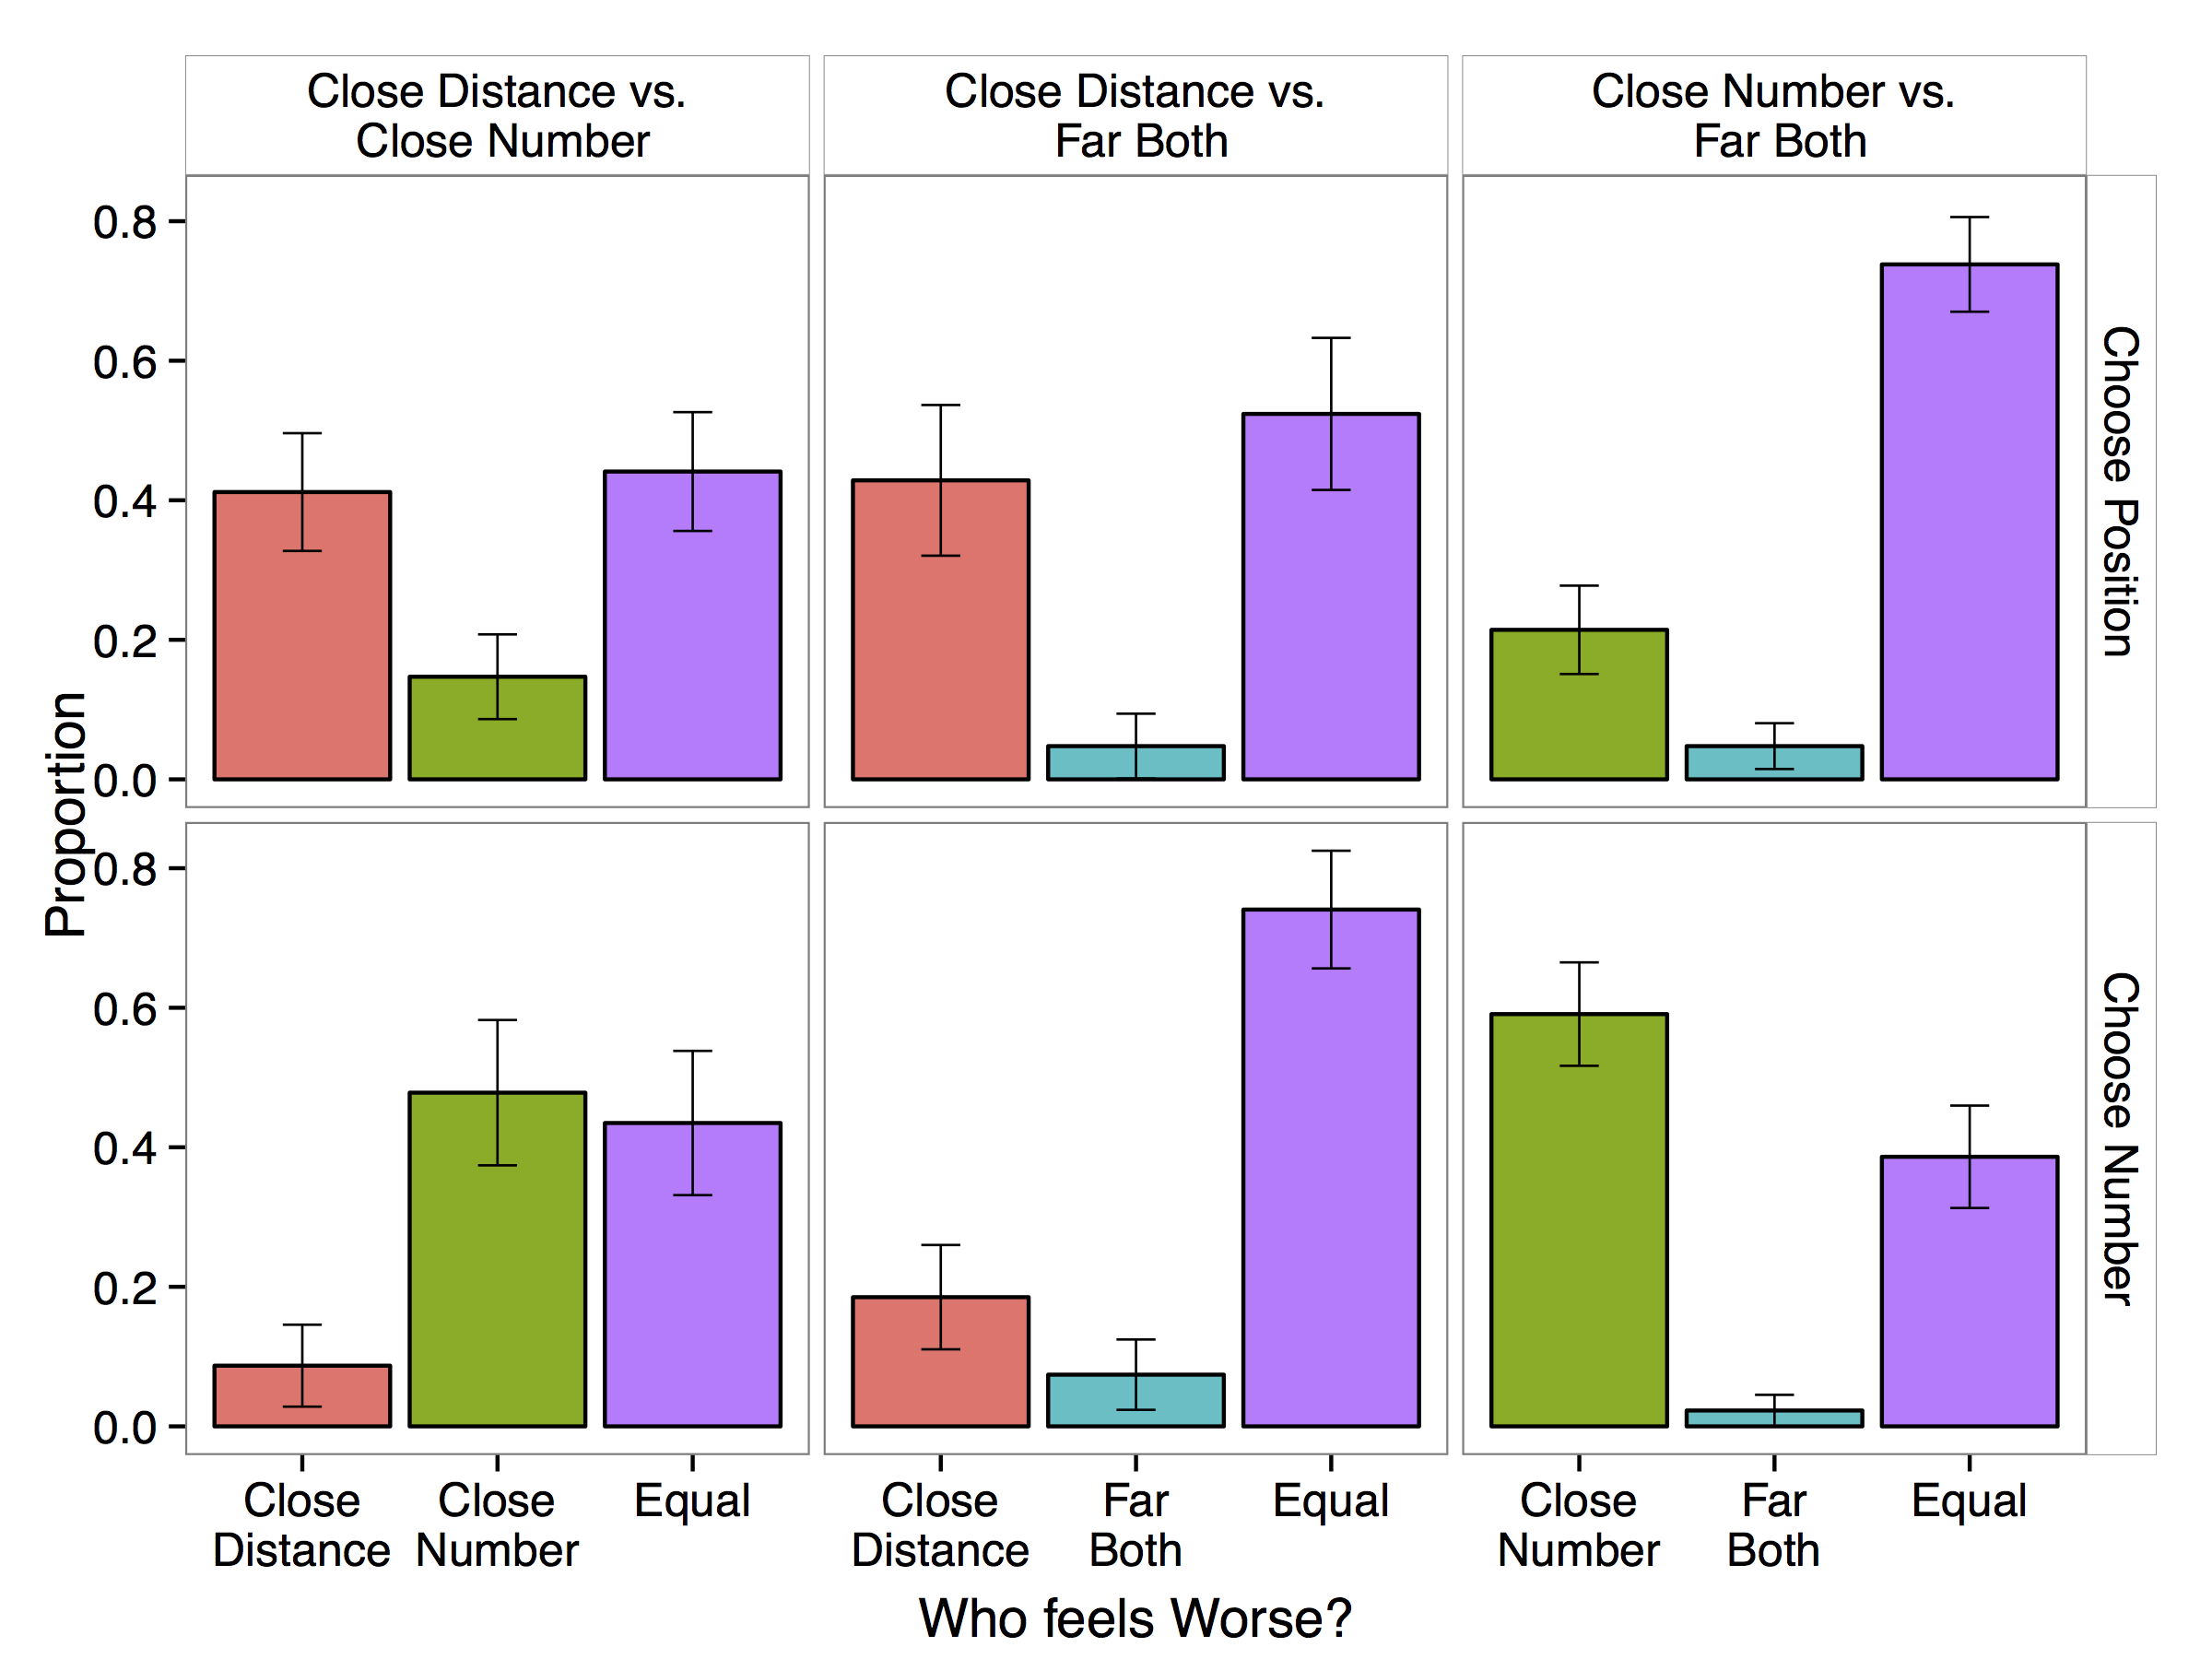
\includegraphics[width=\columnwidth]{images/cardCombined_forcedWorse.png}
\caption{ Expt 2 Results. Proportions of forced choice response. Error bars indicate standard errors. Top row: Choose \textit{Pos}ition condition. Bottom row: Choose \textit{Num}ber condition.}
\label{Expt2ResultFig}
\end{figure}

\subsubsection{Results.} Nine participants were excluded for failing the attention checks. In the \textit{Num} condition, as compared to the far character, the close number character was judged to feel more disappointed ($t(43)=2.81, p=.007$), more regret ($t(43)=2.44, p=.02$), more sadness ($t(43)=2.54, p=.015$) and less relief ($t(43)=2.12, p=.04$), all in the predicted direction. None of the comparisons in the \textit{Pos} condition came out significant. This might suggest that the near-miss effect might not be strong enough to be seen when comparing individual ratings of emotion (in line with the results of Experiment 1).


The results for the forced-choice ratings are shown in Fig. \ref{Expt2ResultFig}. In line with our predictions, in the \textit{Pos} condition, the close distance character was judged to feel worse than the close number character (bootstrapped simulation with 10,000 iterations on full sample, $p=.023$) and the far character (bootstrap $p=.0027$). To a smaller extent, the close number character was judged to feel worse than the far character ($p=.016$). 

By contrast, we see the opposite pattern of results in the \textit{Num} attributions. The close number character was judged to feel worse than the close distance character (bootstrap $p=.0017$) and the far character ($p<.0001$). There was no difference between the close distance and far characters ($p=.17$). 


The results suggest that participants are sensitive to near-misses along multiple dimensions, in this case, both physical closeness and numerical closeness. When given multiple dimensions, participants weight the dimension on which the characters have more illusory control (physical closeness in the \textit{Pos} condition and numerical closeness in the \textit{Num} condition) more than the other dimension. When characters have to pick the physical location of the card, participants attribute more near-miss effects along physical closeness, and when characters have to choose a number (rather than a location), participants attribute more near-miss effects along numerical closeness. Again, it is worth reiterating that characters only have an illusion of control along these dimensions, yet this illusion of control, much like actual control, affects participants' judgments of emotions.





%%%%



\section{Experiment 3: Quantitative modeling of near-misses}
	Experiment 3 involved a meta-analysis of three prior experiments that were designed to examine the features underlying affective cognition in a gambling paradigm. We explicitly model the near-miss effect in a quantitative model of affective cognition.
	
\subsubsection{Participants and procedures.}
	690 participants were recruited across 3 different experiments previously reported in \citeA{OngAffCog}. The basic trial involves watching a character spin a wheel and win the amount on the wheel (Fig. \ref{Expt3ParadigmFig}). Participants then attributed 8 emotions (\textit{happy}, \textit{sad}, \textit{anger}, \textit{surprise}, \textit{disgust}, \textit{fear}, \textit{content} and \textit{disappointment}) to the character after the outcome on the wheel, using 9 point Likert scales. Each participant saw 10 trials, and the payoff and probability structure of the wheels were varied systematically to decorrelate the amount won with the expected value of the wheel. The first experiment only had these basic wheel trials: the second and third had these basic wheel trials intermixed with emotion attribution trials given other stimuli (faces and utterances) instead of wheels. We extracted data from the subset of wheel trials from the second and third experiment, and the entire first experiment, to amass a dataset of 3048 observations from 690 participants to conduct a meta-analysis on.
	
	These experiments were initially designed to test how different features of the situation, namely the amount won and the prediction error, affected participants' attribution of emotion to the character. Yet, because we randomized the position on which the spinner lands, these experiments incidentally provided a valuable dataset to test for near-miss effects.

\begin{figure}[htb!]
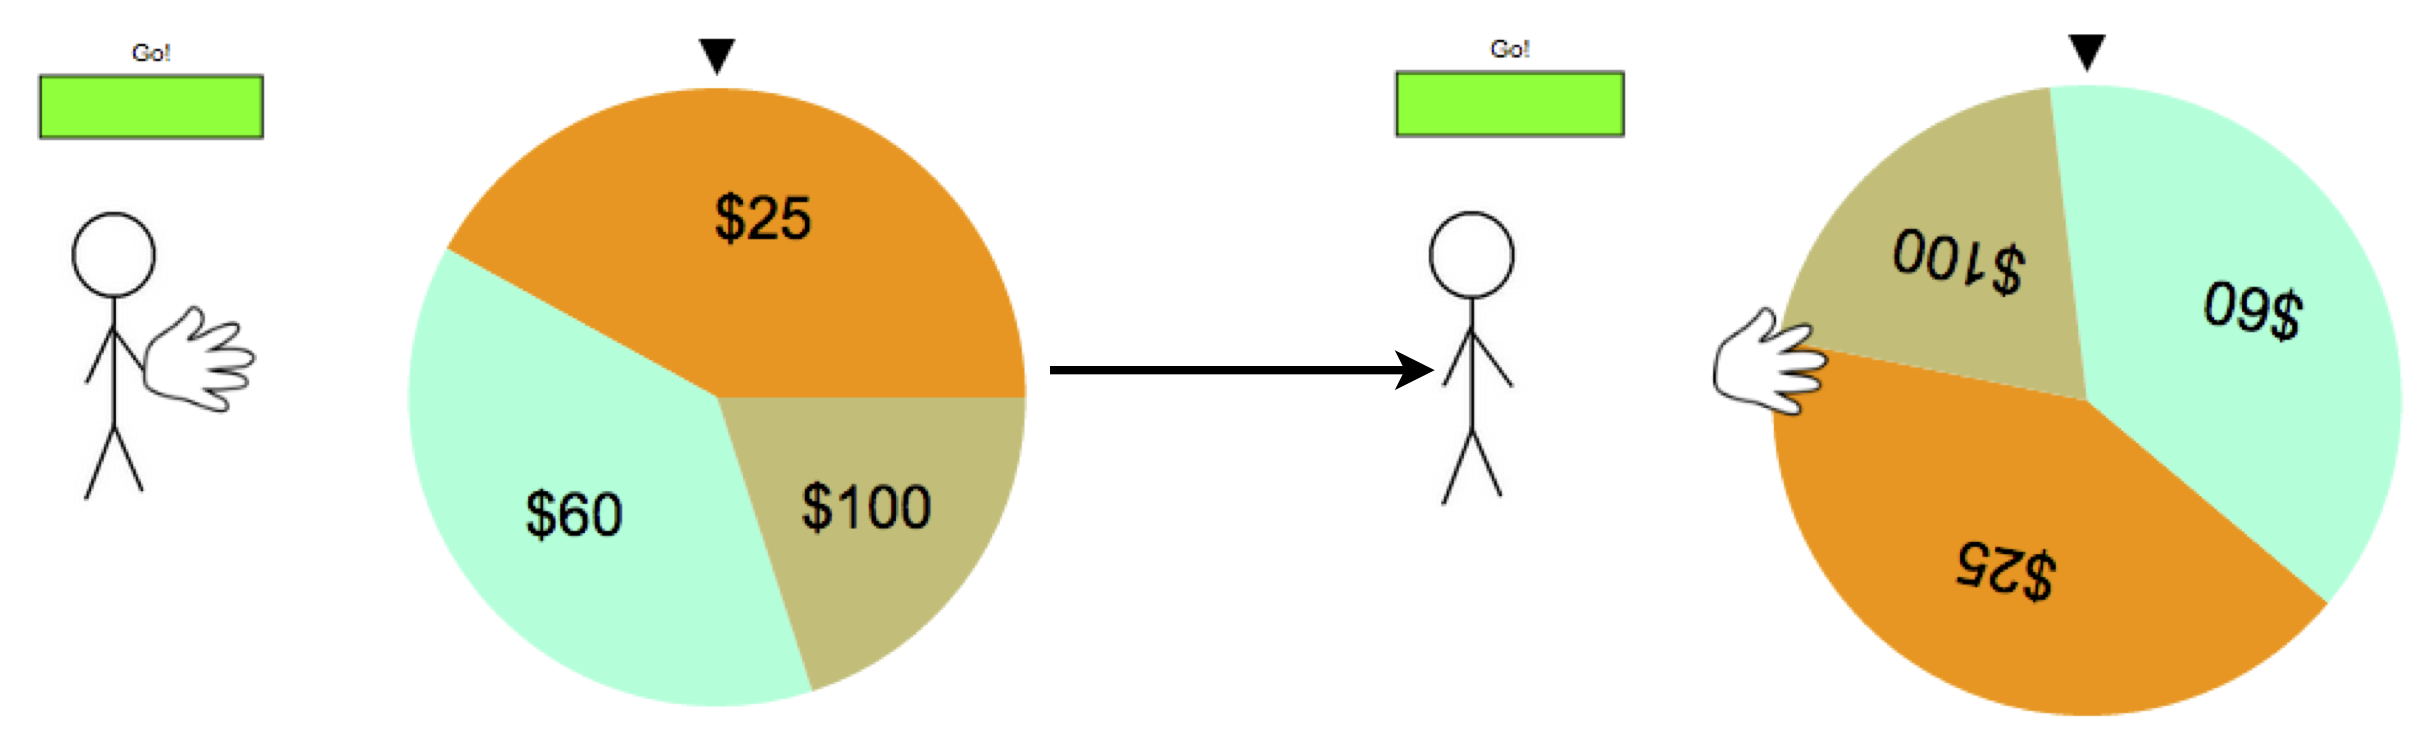
\includegraphics[width=\columnwidth]{images/expt3Paradigm.png}
\caption{ Paradigm for the meta analysis reported in Expt 3. Participants attribute emotions to an agent after the outcome of a spin. After this spin, the agent won \$60 (as indicated by the black pointer), but almost won a lower amount. }
\label{Expt3ParadigmFig}
\end{figure}


\subsubsection{Previous model.} The model we built in \citeA{OngAffCog} incorporated three important features: the amount won (\textit{win}), the prediction error (\textit{PE}), and the absolute value of the prediction error (\textit{absPE}). That is, the emotion E attributed to the agent after event X was:
\begin{align}
E(X) &= b_0 + b_1 \text{win}(X) + b_2 \text{PE}(X) + b_3 \text{absPE}(X) + \epsilon \label{PEModel}
\end{align}
which was a linear combination of \textit{win}, \textit{PE} and \textit{absPE}. The absolute value of the PE was added to test for nonlinear effects, namely, loss aversion, whereby agents will be more sensitive to negative PE values and weigh them more than positive PE values. More discussion can be found in the paper. Eqn. \ref{PEModel} provided the starting point for the model in the following analysis.


\subsubsection{Adding Near Miss to the model.}

%We started with the normalized ending position of where the spinner landed, which ranged from 0 to 1, with 0 indicating the boundary with the sector it would have landed in if the wheel spun less, and 1, the boundary with the sector it would have landed in if the wheel spun more (the wheels spun clockwise). 

Next, we proceeded to define a near miss distance. We calculated a normalized ``distance from the edge" which ranged from 0 to 0.5, with 0 being the boundary edge between the current and closest sector and 0.5 indicating the exact center of the current sector. We then took a reciprocal transform ($1/x$) to introduce a non-linearity that favors smaller distances. Finally, we multiplied the transformed distance with the difference in payment amounts from the current sector to the closest sector. This last component was to account for the difference in utility in the two payoffs. Hence, we had:
\begin{align}
NM(X) &= \frac{1}{\text{distanceToEdge}(X)} * \Delta\text{Payoffs}(X) \label{NMRegressor}
\end{align}
which we added to the model in Eqn. \ref{PEModel}. To illustrate, for the result shown in Fig. \ref{Expt3ParadigmFig}, the distance is approximately .05 (about 5\% of the sector size away from the \$25-\$60 boundary), and the $\Delta$Payoff is 60-25 = 35, as 25 is the next nearest sector.

\subsubsection{Meta analysis results.}

We fit a linear mixed-effects model with the amount won, PE, absPE, and the Near Miss (NM) term (Eqn. \ref{PEModel}, \ref{NMRegressor}) as fixed effects, and random intercepts by participant, wheel, and experiment. There is a significant slope on the NM term ($b = \text{-}3.5 * 10^{\text{-}5}, t(682)=\text{-}2.80, p=0.005$) on happiness. There was no significant differences between NM terms when the next-nearer outcome was positive or negative ($\chi^2(2)=0.13, p=0.94$). To understand the effect size of this NM term, let us consider the slope on win ($b = 0.0405, t(682) = 7.08, p<.0001$), PE ($b=0.036, t(682)=5.86, p<.0001$), and absPE ($b=\text{-}0.015, t(682) = \text{-}2.83, p=.005$) and the example in Figure \ref{Expt3ParadigmFig}. Not considering the near miss effect, and all else being equal, if the result had changed from \$60 to \$100, there will be an \textit{increase} in happiness due to $win$, $PE$ and $absPE$ of $40*(.0405+0.036+(\text{-}0.015)) = 2.46$ points on a 9 point Likert scale. By contrast, if we moved from the center of the \$60 sector to a distance of .01 (1\% of the sector size) away from the \$60/\$100 boundary, there would be a \textit{decrease} in happiness of $40*(1/0.5 - 1/0.01)*(\text{-}3.5 * 10^{\text{-}5}) = 0.137$ points on a 9 point scale. Thus, in this gambling scenario, the effect of a near miss on subjective happiness attributed is on the order of 5\% of the relative happiness of winning the next higher amount. Getting a near miss on the \$60 wheel in Fig. \ref{Expt3ParadigmFig} and narrowly missing the sector \$100 (narrowly missing winning \$40 more) has a subjective cost equivalent to losing about \$2, compared with a far-miss (landing in the center of the sector). This is a small effect relative to actually winning, yet it is a large and not insignificant effect considering that this effect does not depend on changing actual payoffs, but relative closeness. Consider too, that this is a stylized game of chance, with fictional characters and hypothetical gambles, which all might lead to underestimating the size of the true effect in real-life situations like missing planes.

%\red{NDG: i like this result. clear, understandable, and contextualized. it may be that we'll want to include it in our psych rev revisions...}

\section{Discussion}

Near-misses matter emotionally, and in this paper we sought to understand how people factor near-misses into lay theories of emotion. First, we showed that people incorporate near-misses in situations where the agent has no direct control over the outcome, such as the random outcome of a die roll---such numbers are generated by chance and numerical closeness has no actual relevance to the outcome, yet people seem to infer an illusory relevance. Second, when presented with multiple dimensions of closeness, people weight near-misses more when the near-misses fall along a dimension on which agents have illusory control compared to dimensions along which agents do not have such control. Third, using a meta-analysis of three previous experiments with a gambling paradigm designed to study features of affective cognition, we were able to quantitatively model the near-miss effect. This analysis allowed a comparison of the size of the near-miss effect relative to actually winning the next alternative. Additionally, this allows near-misses to be incorporated into more complete models of affective cognition.


As we mentioned in the introduction, though near-miss effects and the broader class of counterfactual effects on emotion seem to be so intuitive, especially to the scientists studying them, there still remains many open questions. How does a near-miss compare with its positive counterpart, the relatively-less-studied ``just-hit"? Although there are some qualitative differences between near-misses and just-hits (such as the frequency of downward and upward counterfactual generation, \citeNP<e.g.>{Roese1997, Sweeny2012}), more work has to be done to study just-hits in a similarly quantitative manner. The model we describe in Experiment 3, for example, takes just-hits into account with the $\Delta$Payoff term, and we found no difference between positive and negative close comparisons (near-miss and just-hits), suggesting a lack of a quantitative difference; however, more in depth work has to be done to confirm this.

The results presented here suggests some interesting properties about near-miss judgments in scenarios where the outcome is randomly-generated. Future work will have to unify this and previous, more general work on counterfactual judgments into quantitative models of affective cognition. The model that we expanded in Experiment 3 already had some consideration of counterfactual judgment with the prediction error and loss aversion terms, yet it is still not the complete story. For example, related work in counterfactuals more generally has shown that the temporal recency of the counterfactual event \cite{Miller1990}, and whether the outcome resulted from an act of omission or an act of commission \cite{Kahneman1982, Landman1987} both affect lay judgments of emotion. How might these features of counterfactuals interact with near-misses and fit into a computational model of affective cognition?


Believe in a fuller 


\section{Acknowledgments}

This work was supported in part by an A*STAR National Science Scholarship to DCO and by a James S. McDonnell Foundation Scholar Award to NDG.


\bibliographystyle{apacite}

\setlength{\bibleftmargin}{.125in}
\setlength{\bibindent}{-\bibleftmargin}

\bibliography{cfDistance}



%	\red{NDG: be clearer here: first, even if people are sensitive to causally-irrelevant dimensions, do they weight causally-relevant ones more? second, is this weighting flexible in the sense that it readily adjusts to contextual factors (not just e.g. physical factors)?}
%	Second, how do observers reason using these distance dimensions? In any particular situation, there could be more than one dimension of closeness, although not all of them would be causally-relevant, or otherwise relevant to the task at hand. Depending on the context, different dimensions of distance should matter to different extents. For example, if one was flipping over numbered cards trying to match a target number, is the proximal distance of the chosen card to the target card relevant? Is the numerical distance of the chosen card to the target card relevant? For the former, yes, and for the latter, much less so. What about if one was guessing a number and writing it down instead? In that case, numerical closeness should matter more. In Experiment 2, we show that observers are sensitive to contextual information (the rules of the game and the information that is presented) that changes the relevance of different distances in a random card-guessing task, and spontaneously alter their judgments during the task when presented with additional information.
%\textcolor{red}{(to discuss with Noah more on this point. action-outcome contingency.)} %not sure how to add this in.
	
	
	
	%One proposed \textit{causally-relevant} explanation for the near miss effect is that of controllability: Mr Tees could easily think of actions he could have done differently (``if only I woke up ten minutes earlier") that would have led to him catching the plane. \red{NDG: controllability isn't explained clearly here, and no alternative is given, so it isn't clear why you mention it.}


%% Can this paragraph fit here? or should it belong between the end of the Intro and the start of Expt 1, in a section called "Predictions" (that was the way I had it initially).
%	Based upon findings from previous work \cite{Kahneman1982, Johnson1986, Gleicher1990}, we can list several predicted properties of near-miss effects. See Fig. \ref{PredictionFig} for an illustration, where we have included both near-miss and just-hit effects, although we focus on the former in this paper. First, the near-miss effect should be \textit{non-linear} with respect to distance to the desired outcome---the near miss effect should only occur at small distances, and should matter increasingly more with increasingly smaller distances. Second, the magnitude of the near-miss effect should be \textit{small but proportional} to the difference between the desired and undesired outcome.
%\red{NSG: these properties are predicted from your graph, but it's not clear where your graph came from -- it sounds like you're just making them up...}
%
%\begin{figure}[htb!]
%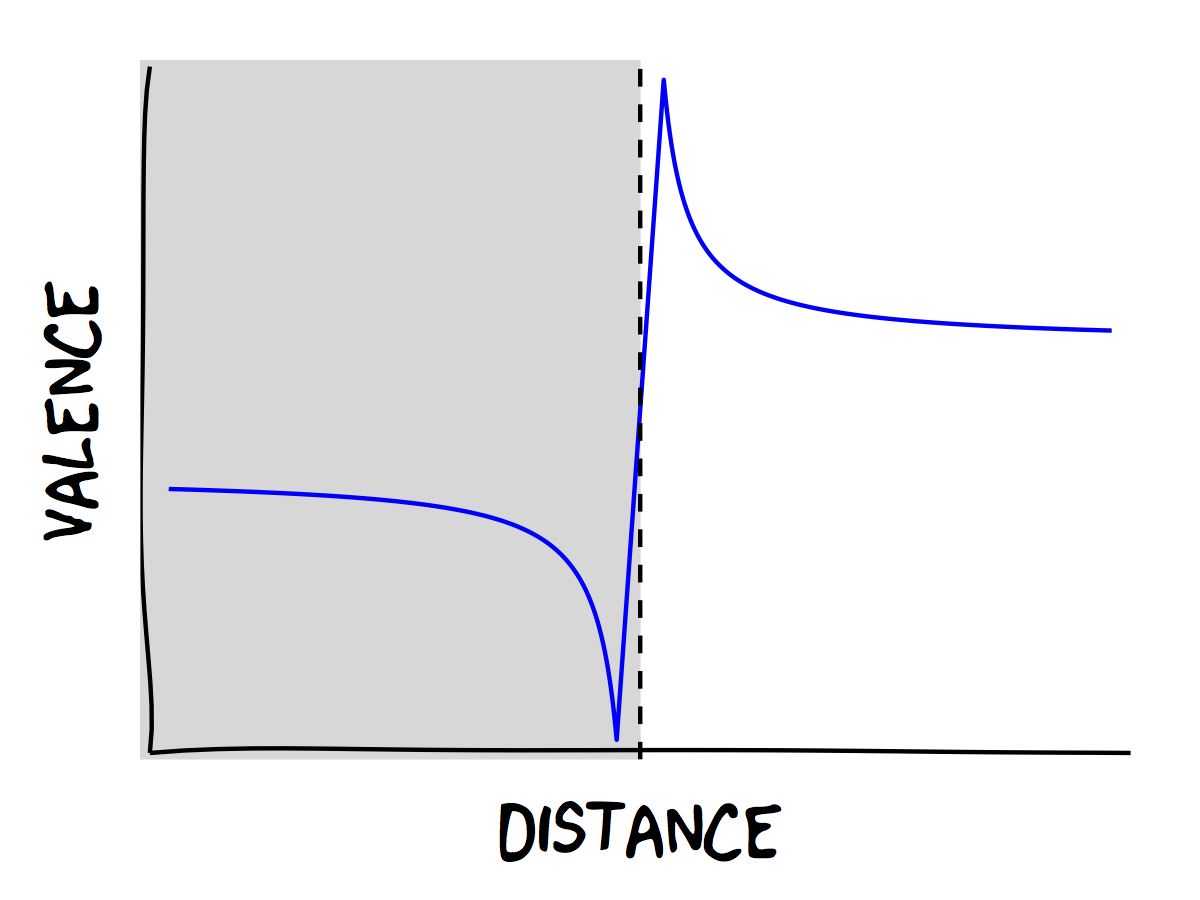
\includegraphics[width=\columnwidth]{images/predictionFig.png}
%\caption{ Prediction. A plot of emotional valence against ``distance" to the counterfactual world, where the unshaded region represents the desired outcome, and the shaded region, the ``miss" region. Near misses and ``just-hits" are predicted to be non-linear variations of valence at small distances to the miss-hit boundary.}
%\label{PredictionFig}
%\end{figure}



% be a little less vague 
%The distances that separate the desired-but-unattained counterfactual world from the current world.

% define dimensions

%	There however, remains many open questions regarding the nature of the near-miss effect, and in this paper we address three of them. First, what are the dimensions of distance that observers judge to be relevant to an agent's emotions?  The answer most commonly proposed by the current literature asserts that people should consider causally-relevant dimensions, like the amount of time one misses a plane by. This would predict that people should not exhibit near miss effects in their lay theory when considering games of chance, or random events, as the causal process that generated the outcomes are based on chance. However, previous work has shown that gamblers persist more after near misses, showing a near-miss effect on motivation even though the outcome of games like slots are independent of the gambler's actions \cite{Kassinove2001, Reid1986}. In Experiment 1, we show that observers readily judge an agent who ``narrowly misses" on a die game (by rolling a number close to the target number) to feel worse than one who misses by a larger amount, even though outcomes on a die game are not ordered like the number line. This suggests that observers may also consider causally-irrelevant dimensions

%Observers seem to consider causally-irrelevant dimensions of distance as well, when a causally-relevant dimension does not exist.






%Spell out relevant and irrelevant. Deeper theory.

%Nearness compared to actual outcome differences



%Hmm maybe not the best example: even if the 7 mins was reduced to 0, they wouldn't necessarily have won.

%	Argentina nearly won the 2014 FIFA World Cup Final, conceding the only goal of the match with barely 7 minutes left in extra time, but as the above idiom morbidly points out\footnote{Points in horseshoes are scored based on distance thrown horseshoes land from the target stake. Thrown hand grenades, in contrast, do not need to hit their target to be effective.}, close in this case, does not count. However close they were, they did not win. However, as Argentinian supporters would attest, close does matter---\textit{emotionally}.



%	Though we live in only one of many possible realizations of the world, our mental lives---and consequently, our emotional lives---are constantly spent exploring other possible worlds via counterfactual thinking \cite{Bryne2002, Gleicher1990, Johnson1986, Roese1997}. ``Near-miss" or close counterfactual comparisons in particular, are so mentally engaging because these possible worlds had almost happened. Consider \citeA{Kahneman1982}'s classic example of missing a plane by 5 minutes, as opposed to 30 minutes: people consistently and reliably judge the person who narrowly missed his plane to feel much worse than the one who missed it by a wider margin. One proposed reason is that it is much easier to generate possible counterfactual antecedents that would have resulted in the counterfactual consequent of catching the plane. The near-miss character could easily generate counterfactuals like ``If only I woke up 5 minutes earlier" or ``if only I had packed my bag the night before", that would result in the consequent ``then I would have caught my plane". If the counterfactual world is somehow \textit{closer} to the current world, then perhaps the counterfactual world would only require a smaller change in the causal chain that led up to the current world in order to be realized.
%
%	Previous research has identified some of the impact of closeness on counterfactual thought \cite{Kahneman1990, Teigen1996}. Closeness increases the activation of counterfactual thought, by increasing the salience of the counterfactual world \cite{Kahneman1982, Roese1997}, and additionally also amplifies the affective consequence of the counterfactual comparison \cite{Johnson1986, Kahneman1982}. Narrowly missing a plane or a World Cup Title feels far worse than missing it by a large margin. 
%	
%	Yet, there remains many open questions regarding the nature of these distances. What are the relevant dimensions of closeness that people incorporate into their lay theories of the world, and into their lay theories of emotion? Intuitively, people should consider only causally-relevant dimensions, like the amount of time one misses a plane by. However, anecdotally we are reminded of many instances where a (randomly-generated) lucky draw number is announced, and the holder of a (randomly-assigned) lucky draw ticket that is off by 1 number expresses extreme negative emotions. Given the random nature of this game, his number is not any ``closer" to reality than any other number in the set of possibilities.
	
	

%\subsection{Outline of paper:}
%\begin{enumerate}
%\item Lay out near miss predictions. Noticably: clearly, on both win and lose sides.
%\item Expt 1: just show it with vignettes, where distance is causally related to outcome
%\item Expt 2: show it with die vignettes, where distance is irrelevant
%\item Expt 3: card task, show that the relevant dimension can be tweaked
%\end{enumerate}
%
%
%
%\subsection{Contributions:}
%\begin{enumerate}
%\item ToE takes into account near misses -- but along what dimensions?
%\item show robustly that it considers both neg and positive misses (expt1)
%\item show that it considers irrelevant distances
%\item 
%\end{enumerate}
%
%Any similarity, causal counterfactual
%control-relevant (exploitable) causal counterfactual
%covert utility differences



%%% Expt 2 other conditions

%\red{NDG: contrary to expt 1??}
%, and Two-Step-Position (\textit{Two-Pos}; N=100).

%\red{NDG: it's hard to follow this section because the condition labels, etc are cryptic. how about ``close distance'', ``far both'', ``close number''. and ``position relevant'', ``number relevant''? or something that ties more closely to control -- here it's controllability i think, not simple relevance?}


%We predicted that in the \textit{Pos} condition, proximity would be judged to be a more relevant dimension of closeness than numerosity, and so the close distance character would be judged to feel worse than the close number character, although the close number character would, to a lesser extent, be judged to feel worse than the character who chose the far card. In the \textit{Num} condition, on the other hand, proximity is irrelevant, and so we predicted that the close number character would be judged to feel the worst, and there would be no difference between the close distance character and the far character. \red{NDG: why?? this doesn't seem to follow from any theory laid out so far in the paper.}

%The visual description that participants saw was similar to the \textit{Pos} condition. 

%\red{NDG: the Two-Pos condition is hard to follow.}
%The Two-Step-Position (\textit{Two-Pos}) condition was similar to the \textit{Pos} condition, except that after characters picked their cards but \textit{before} the winning card is revealed, participants make one set of emotion attributions and one forced-choice on who felt worse. Following this, the winning number 10 is revealed, and then participants make another set of attributions. Hence, participants in this condition made two sets of attributions, one before the location of the winning card is revealed (\textit{Two-Pos-BeforeReveal}), and once after (\textit{Two-Pos-AfterReveal}).

%\subsubsection{Predictions.}

%The \textit{Two-Pos} condition has an interesting twist. Prior to finding out the position of the winning card, position is still a more relevant dimension than numerosity because of the context, but participants do not yet know the position of the winning card, which makes it impossible to judge closeness based on proximal distance. In this attribution, observers should make judgments based on numerosity. There would also be no difference between the proximally close and the far characters, and we predicted that the numerically close character will be judged to feel the worse of them all (i.e., \textit{Two-Pos-BeforeReveal} results should be similar to \textit{Num}). However, after finding out the position of the winning card, proximal closeness becomes possible to judge, and so we should expect to see the proximally close character being judged as feeling the worst (\textit{Two-Pos-AfterReveal} results should be similar to \textit{Pos}).


%results

%For the \textit{Two-Pos-AfterReveal} attributions, the proximally-close character was judged to feel more disappointment ($t(31)=3.25, p=.003$), more regret ($t(31)=3.56, p=.001$), more sadness ($t(31)=2.76, p=.01$) and less happiness ($t(31)=2.67, p=.01$) compared to the numerically-close character. The proximally-close character was also judged to feel more disappointment ($t(33)=2.73, p=.01$), more regret ($t(33)=4.24, p=.0001$), more sadness ($t(33)=2.99, p=.005$), less happiness ($t(33)=2.49, p=.018$), and less relief ($t(33)=2.77, p=.009$) than the far character.

%For the \textit{Two-Pos-AfterReveal} judgments, we find them to be qualitatively similar, in line with our predictions: the proximally-close character was judged to feel worse than the numerically-close character ($p=.0001$) and the far character (bootstrap $p=0$ as there were no observations for the far character feeling worse). The numerically-close character was not judged, however, to feel worse than the far character ($p=.41$).

%In the \textit{Two-Pos-BeforeReveal} attributions, the numerically-close character is judged to feel worse than the proximally-close character ($p=.004$) and the far character ($p=.0001$), while there is no difference between the proximally-close and far characters ($p=.13$).

%The results suggest that observers are sensitive to multiple dimensions, in this case, both proximal closeness and numerical closeness, and are able to flexibly judge which is the dimension that is more relevant to the task. When characters have to pick the physical location of the card, participants attribute near-miss effects along proximal closeness, and when characters have to choose a number (rather than a location), participants attribute near-miss effects along numerical closeness. However, participants still judge near misses along numerical closeness (but to a much smaller extent) when numerosity is not a task-relevant dimension, supporting the results from Experiment 1. 
%In the Two-Step-Before attribution, for example, numerical closeness is irrelevant, but the position of the winning card is unknown, so perhaps participants are judging near-misses based on the only information available.

%\red{NDG: hmm. these results don't seem to add much to the previous lit, do they?}







%%%%% This is the basic vignette experiment %%%%%
%
%\section{Experiment 1: Vignettes}
%In Experiment 1, participants made attributions of emotion to characters in ``near-miss" or ``just-hit" vignettes.
%
%\subsubsection{Materials.} We generated 6 vignettes that involved a dimension of ``distance" which was relevant to the outcome. There were two characters in each vignette. For example, in the ``freeGift" vignette, participants read about Scott and Frank who were both in line for a free brand new vacuum cleaner. Scott was 2nd in line when they ran out of free gifts, while Frank was number 10 when they ran out of free gifts. The possible distances shown were drawn from the following possible values: \{-50, -10, -2, 2, 10, 50\}, where negative values indicates not making the desired outcome. The example described above had distances of -10 and -2. The other vignettes involved: 2) just missing a plane, 3) getting tickets for a concert, 4) making it to a gelato shop before closing time, 5) getting admitted to a course at the local community college and 6) running out of paint when painting a fence.
%
%\subsubsection{Participants.} We recruited 100 participants through Amazon's Mechanical Turk and paid them for completing the experiment. All experiments reported in this paper were conducted according to guidelines approved by the Institutional Review Board at Stanford University.
%
%\subsubsection{Procedures.} Participants viewed each of the six vignettes in a random order. After each vignette, they answered several attention check questions, before rating how each character in the story felt, along six emotions: \{happiness, sadness, contentment, disappointment, relief, and regret\}. After they attributed emotions to both characters, participants made a forced choice rating: which character felt happier? They were also given a neutral option: ``Both feel equally happy".
%
%
%\begin{figure}[htb!]
%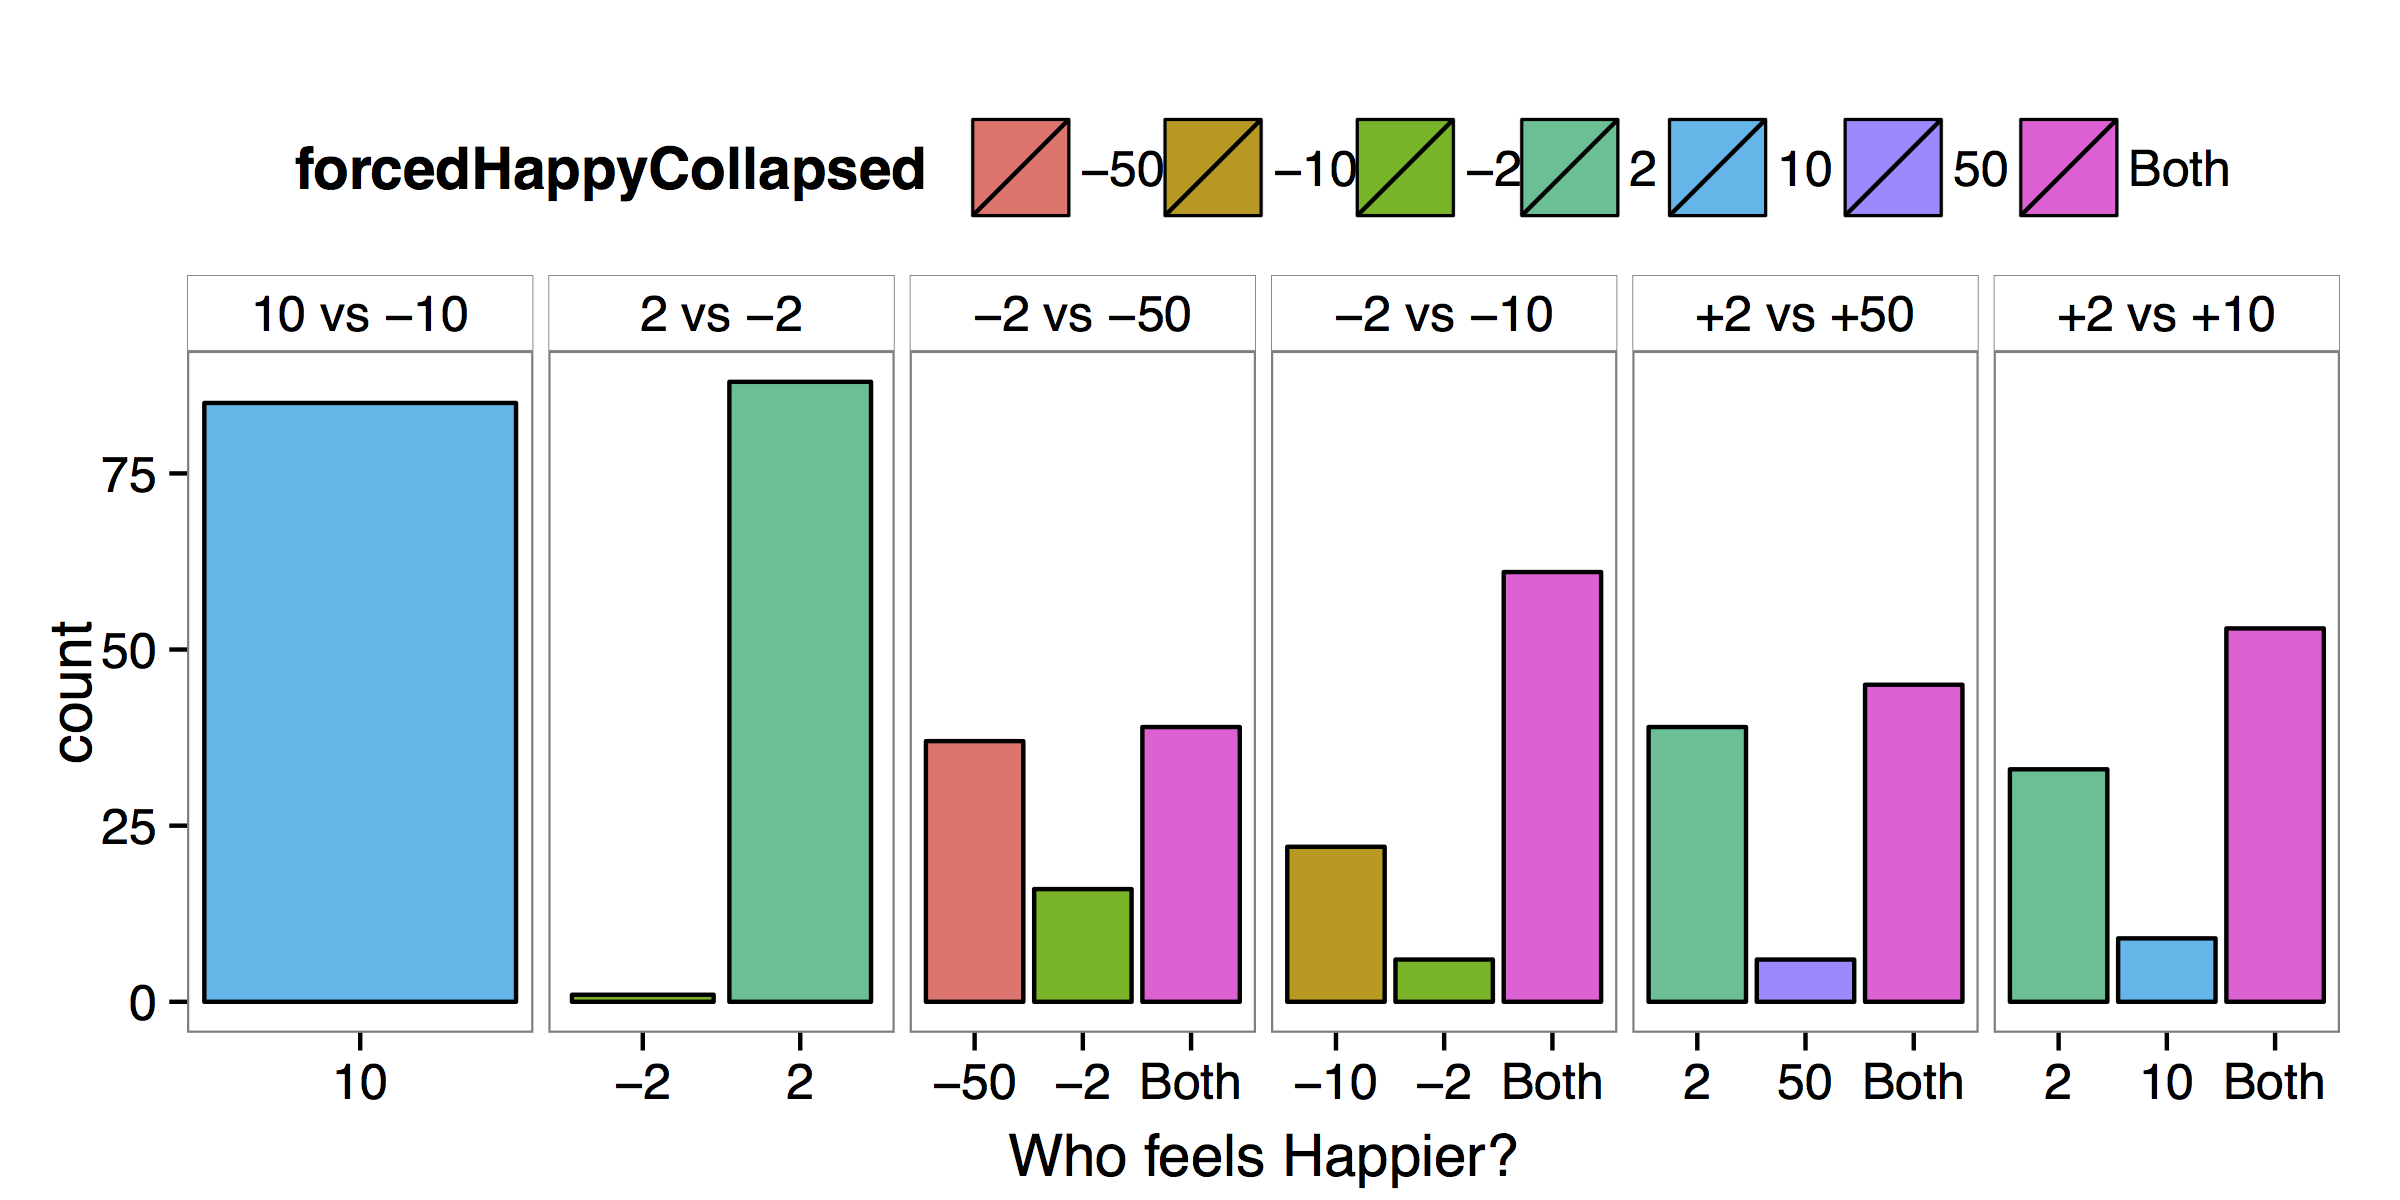
\includegraphics[width=\columnwidth]{images/vignettes_forcedHappy.png}
%\caption{ Expt 1 Results. Proportions of forced choice response to ``Who feels happier?". Error bars indicate standard errors. Answers are labeled with the distance of the character's outcome. E.g., in the right-most panel, more people judged the character who just made the outcome (+2) to be happier than the character who made it by a larger margin (+10).}
%\label{Expt1ResultFig}
%\end{figure}
%
%%%%% STATS
%
%\subsubsection{Results.} Post-hoc analysis showed that results were similar across five of the vignettes\footnote{The only anomaly was the fence painting vignette. In the critical comparison in that vignette, X ran out of paint with just 2 inches of fence left, while Y ran out with 10 inches left. Although we predicted that the near-miss character (X) would feel worse, painting a fence involves a persistent product rather than a once-off event: X could return to fence in the future, and he only needs to paint 2 more inches then. In this case, the more distance, the better. We excluded this vignette from the analyses.}: the character that experienced the near-miss (-2) was rated to feel worse than the character that experienced a further-miss (-10, -50) (STATS), and the character that just made the outcome (+2) was rated to feel better than the character that made the outcome by a large margin (+10, +50) (STATS).
%
%The forced choice results are given in Fig. \ref{Expt1ResultFig}. Across the win-lose comparison (left two panels), all participants rated the character who obtained the outcome to be happier. Across lose-lose comparisons, far fewer participants rated the near-miss character as feeling happier (STATS), and across win-win comparisons, far more participants rated the just-hit character as feeling happier (STATS). We note that a large proportion of participants chose the neutral option, and this proportion is higher than than the near-miss/just-hit judgments. 
%
%% 
%\textcolor{red}{\textit{COMMENT: do we interpret the high proportion of "Both" as meaning that it's a weak effect? or that there are individual differences, and majority of Ps might not be sensitive to this?}}
%
%
%%%%%% End Vignette Experiment


\end{document}
